\documentclass[aspectratio=169,10pt]{beamer}
% Session 1 slides. Same preamble as the kick-off deck. Change aspectratio to 43 if needed.

% --- If you prefer, replace this block with \input{preamble}.
\usepackage[utf8]{inputenc}
\usepackage[english]{babel}
\usepackage{amsmath,amssymb}
\usepackage{xcolor}
\usepackage{graphicx}
\usepackage{hyperref}
\usepackage{booktabs}
\IfFileExists{lmodern.sty}{\usepackage{lmodern}}{}
\usepackage{tikz}
\usetikzlibrary{positioning,arrows.meta,calc,fit,decorations.pathreplacing}
\usepackage[font=footnotesize]{caption}

\definecolor{color1bg}{HTML}{005e9e}
\setbeamercolor*{palette primary}{fg=white,bg=color1bg}
\setbeamercolor*{block title}{bg=color1bg,fg=white}
\setbeamertemplate{caption}[numbered]
\definecolor{color2bg}{HTML}{003a63}
\setbeamercolor{block title alerted}{bg=color2bg,fg=white}
\setbeamercolor{block body alerted}{bg=color2bg!8}
\setbeamercolor{alerted text}{fg=color2bg}
\beamertemplatenavigationsymbolsempty
\setbeamertemplate{footline}[frame number]

% --- One blue for all titles: the blue of the title page (Beamer's default structure blue).
\definecolor{titleblue}{rgb}{0.2,0.2,0.7}
\setbeamercolor{title}{fg=titleblue}
\setbeamercolor{subtitle}{fg=titleblue}
\setbeamercolor*{frametitle}{fg=titleblue}
\newcommand{\sectiontitle}[1]{{\Huge \textbf{\textcolor{titleblue}{#1}}}}

% --- Change marker: text changed since the previous version is in \chg{...} (bold).
% --- Once checked, switch off by uncommenting the second line.
\newcommand{\chg}[1]{\textbf{#1}}
% \renewcommand{\chg}[1]{#1}

\newcommand{\mono}[1]{\texttt{#1}}

\title[LLMs for Social Science Research]{\large \textbf{Large Language Models for Social Science Research} \\
    \textit{Session 1: Setting Up an Agentic Research Project}}
\author[H. Subtil]{\textbf{Hugo Subtil}}
\institute{University of Zurich \\[0.4cm] \chg{\footnotesize Course repository: \url{https://github.com/subtilhugo/uzh-llm-socsci-2026}}}
\date{14 October 2026}

\begin{document}
\frame{\titlepage}

% ============================================================================
% PART 1: BEFORE WE START
% ============================================================================

\begin{frame}[plain]
  \centering
  \vfill
  \sectiontitle{Before We Start}\\[0.4cm]
  {\Large \textit{9:25 -- 9:35}}\\[0.3cm]
  {\large \chg{The idea of this session, and why it is debatable}}
  \vfill
\end{frame}

\begin{frame}{An Economics Paper, Produced Autonomously}

\vspace{0.1cm}
\begin{columns}[T]
\column{0.58\textwidth}
\begin{itemize}
    \item An AI system picks a policy question, finds public data, writes the code, estimates the effect, writes the paper.
    \vspace{0.1cm}
    \item No human in the loop.
    \vspace{0.1cm}
    \item The project: \textbf{Autonomous Policy Evaluation (APE)}, Social Catalyst Lab, \textbf{University of Zurich}. Two buildings from here.
    \vspace{0.1cm}
    \item \chg{Hundreds of papers (900+ by spring 2026)}, judged by LLM referees in a tournament against published economics papers.
\end{itemize}

\column{0.38\textwidth}
\vspace{0.8cm}
\centering
{\Large \textcolor{titleblue}{$\blacktriangleright$} \textbf{\chg{Video, 2 minutes}}}\\[0.25cm]
{\footnotesize Posted on LinkedIn by the project's author, \chg{February 2026}}\\[0.5cm]
{\footnotesize \url{https://ape.socialcatalystlab.org}}
\end{columns}

\end{frame}

\begin{frame}{The Author's Own Reading: Two Worlds}

\vspace{0.1cm}
\begin{columns}[T]
\column{0.46\textwidth}
\textbf{World 1.} This is real research. But it has nothing to do with my expertise. I cannot evaluate it. Some other human expert has to.

\column{0.46\textwidth}
\textbf{World 2.} This is not real research. I just produced a negative externality by polluting the information environment.
\end{columns}

\vspace{0.5cm}
\textbf{His conclusion.} In a world of machine-speed papers, we have a problem either way.
\alert{\textbf{Generation speed $\gg$ verification speed.}} This was never the case historically.
Anybody, with no expertise, can now produce a paper that looks legitimate at first glance.

\vspace{0.3cm}
Open questions he lists: matching in the academic labour market, credit attribution. ``I don't have the answers.''

\vspace{0.3cm}
\textbf{Neither do I. But we can push this a little further, and it changes what we do in this room.}

\end{frame}

\begin{frame}{Pushing It Further (1): The Bottleneck Moved}

\vspace{0.1cm}
\begin{columns}[T]
\column{0.55\textwidth}
\textbf{His two worlds have one consequence in common.}
Real research he cannot evaluate, or pollution: either way, the scarce resource is no longer production. It is \alert{qualified verification}. The bottleneck moved from \emph{doing} to \emph{judging}.

\vspace{0.3cm}
\textbf{Why did this never happen before?}
\begin{itemize}
    \item Verification was always slow. But generation was slow too.
    \item The cost of writing a paper was a \textbf{filter}: you did not write one you did not believe in.
    \item It was also a \textbf{signal} of competence, in Spence's sense: costly, hence informative.
    \item Peer review was calibrated for a world where submitting cost a year.
\end{itemize}

\column{0.42\textwidth}
\centering
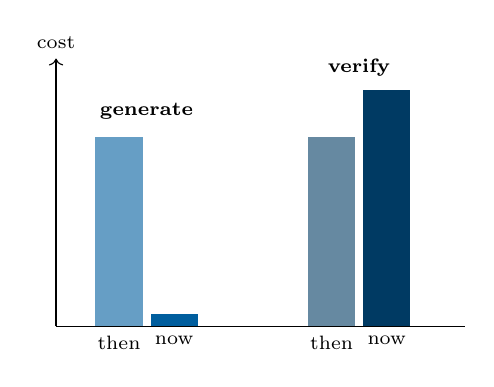
\begin{tikzpicture}[font=\scriptsize, x=1cm, y=1cm]
  \draw[->] (0,0) -- (0,3.4) node[above] {cost};
  \draw (0,0) -- (5.2,0);
  \fill[color1bg!60] (0.5,0) rectangle (1.1,2.4);
  \fill[color1bg]    (1.2,0) rectangle (1.8,0.15);
  \node[below] at (0.8,0) {then};
  \node[below] at (1.5,0) {now};
  \node[above] at (1.15,2.5) {\textbf{generate}};
  \fill[color2bg!60] (3.2,0) rectangle (3.8,2.4);
  \fill[color2bg]    (3.9,0) rectangle (4.5,3.0);
  \node[below] at (3.5,0) {then};
  \node[below] at (4.2,0) {now};
  \node[above] at (3.85,3.05) {\textbf{verify}};
\end{tikzpicture}

\vspace{0.2cm}
{\footnotesize The cost of generating falls towards zero. The cost of verifying \emph{rises}: you now have to check the pipeline, not only the text.}
\end{columns}

\end{frame}

\begin{frame}{Pushing It Further (2): Verification at Machine Speed}

\vspace{0.1cm}
\textbf{This is not hypothetical. People have already looked at the APE papers from the outside.}

\vspace{0.2cm}
\begin{itemize}
    \item \textbf{Cunningham (2026)} went through 651 APE papers: systematic p-hacking patterns in the choice of specifications and in what gets reported.
    \vspace{0.1cm}
    \item \textbf{Ning (2026)} compared 912 APE papers with 41 papers from the \emph{AER} and \emph{AEJ: Economic Policy}, with the same LLM judge as the APE tournament: the AI papers lose, and the largest gap is on \emph{ideation}, not execution.
\end{itemize}

\vspace{0.3cm}
\textbf{The detail that matters for us.} To verify 651 papers, Cunningham used a large language model. The APE tournament itself is judged by LLM referees.

\vspace{0.25cm}
{\centering {\Large \alert{\textbf{Who verifies the verifier?}}}\par}

\vspace{0.25cm}
Verification at machine speed is possible. It is also the same machine. The chain has to end with a human who understands what was done.

\vspace{0.3cm}
{\scriptsize Cunningham, S. (2026), \emph{causalinf.substack.com}, ``Do AI agents writing full manuscripts at the Social Catalyst Lab p-hack?''.
Ning, L. (2026), ``The ideation bottleneck'', arXiv:2604.03338.}

\end{frame}

\begin{frame}{Pushing It Further (3): The Dependence Trap}

\vspace{0.1cm}
\textbf{The capacity to verify is produced by doing.}
If nobody does the thing any more, then within one cohort nobody can check the thing. And when nobody can check, everybody depends on whoever still can.

\vspace{0.5cm}
\begin{columns}[T]
\column{0.46\textwidth}
\textbf{The Covid version.}
Countries that had stopped making basic goods (masks, paracetamol) found they could not make them when it mattered. Not because it is hard. Because they had handed the know-how to someone else.

\column{0.46\textwidth}
\textbf{The academic version.}
The senior PI who delegates everything to research assistants and stops checking. When it breaks, it is \emph{their} name on the paper.

\vspace{0.2cm}
\alert{\textbf{Responsibility does not delegate.}}
\end{columns}

\vspace{0.5cm}
An agent is a research assistant who never gets tired, never says ``I am not sure'' unless you ask, and bears no responsibility at all.

\end{frame}

\begin{frame}{The Trade-off, and Why It Is Yours to Make}

\vspace{0.1cm}
\begin{columns}[T]
\column{0.46\textwidth}
\textbf{Short term, individual.}
Delegating everything is rational. You will produce more, faster. The productivity imperative is real, and your career is short.

\column{0.46\textwidth}
\textbf{Long term, collective.}
Expertise is a common-pool resource. Every person who stops understanding depletes it a little. Nobody feels it until it is gone.
\end{columns}

\vspace{0.5cm}
\textbf{And the feeling of productivity is not productivity.}
In a randomised trial by METR (2025), experienced open-source developers were \alert{\textbf{19\% slower}} with AI tools on their own codebases, while believing they had been about 20\% faster. A narrow setting, but keep the gap between the feeling and the measurement.

\vspace{0.5cm}
\centering
\textbf{I am not going to pretend this trade-off is balanced. It is your choice. Here is mine.}

\vspace{0.3cm}
{\scriptsize Becker et al. (2025), ``Measuring the impact of early-2025 AI on experienced open-source developer productivity'', METR. 16 developers, 246 tasks.}

\end{frame}

\begin{frame}{My Position, and Three Rules for This Workshop}

\vspace{0.1cm}
\begin{alertblock}{Where I stand}
\centering
I am not here to teach you the technique. I am here to show you how to delegate it. \\
But I think we have a moral obligation to understand what we delegate. \\
Otherwise we will not know how to do it, and when nobody knows, we all depend on someone else.
\end{alertblock}

\vspace{0.4cm}
\begin{enumerate}
    \item \textbf{You delegate execution, never understanding.} You must be able to explain every file in your project.
    \vspace{0.2cm}
    \item \textbf{Read before you accept.} Every output is a draft. Every session has a mandatory manual check.
    \vspace{0.2cm}
    \item \textbf{Stop when you no longer know what it is doing.} Supervising agents is work. Fatigue is the signal to stop, not to accept faster.
\end{enumerate}

\vspace{0.4cm}
\centering
\textbf{This is exactly why we do not start with a chat. We start with a folder.}

\end{frame}

\begin{frame}{\chg{This Morning}}

\vspace{0.2cm}
\setlength{\leftmargini}{2.4cm}
\begin{enumerate}
    \item[\textcolor{gray}{\textbf{9:00--9:25}}] \textcolor{gray}{Installation clinic.}
    \vspace{0.15cm}
    \item[\textcolor{gray}{\textbf{9:25--9:35}}] \textcolor{gray}{\chg{Before we start.}}
    \vspace{0.15cm}
    \item[\textbf{9:35--9:50}] \chg{\textbf{An agentic research project.} What it is, why a folder, what is in it.}
    \vspace{0.15cm}
    \item[\textbf{9:50--10:25}] \textbf{Live demo.} The example project, from an empty folder to a first commit.
    \vspace{0.15cm}
    \item[\textbf{10:25--10:40}] Break.
    \vspace{0.15cm}
    \item[\textbf{10:40--11:40}] \textbf{Hands-on.} The same thing, on your project. Worksheet, steps 1 to 8.
    \vspace{0.15cm}
    \item[\textbf{11:40--12:00}] \textbf{Debrief.} Three screens, the errors we found, what to bring on 28 October.
\end{enumerate}

\end{frame}

% ============================================================================
% PART 2: THE AGENTIC PROJECT
% ============================================================================

\begin{frame}[plain]
  \centering
  \vfill
  \sectiontitle{An Agentic Research Project}\\[0.4cm]
  {\Large \textit{9:35 -- 9:50}}\\[0.3cm]
  {\large From a chat that forgets to a folder that remembers}
  \vfill
\end{frame}

\begin{frame}{Chat vs Agent}

\vspace{0.1cm}
\begin{columns}[T]
\column{0.46\textwidth}
\textbf{A chat}
\begin{itemize}
    \item You paste; it answers; you copy.
    \item It sees what you paste, nothing else.
    \item It forgets everything when you close the tab.
    \item It cannot open your PDF, run your script, or look at your data.
\end{itemize}

\column{0.46\textwidth}
\textbf{An agent}
\begin{itemize}
    \item It works \textbf{inside a folder} on your machine.
    \item The loop: \textbf{read} files $\rightarrow$ \textbf{run} commands $\rightarrow$ \textbf{write} files $\rightarrow$ report.
    \item It asks permission before each action that changes something.
    \item Claude Code, Gemini CLI, Codex: same idea, different vendors.
\end{itemize}
\end{columns}

\vspace{0.6cm}
\textbf{The permission prompt is the only thing that separates an assistant from an unsupervised intern.} Keep it on. Read it.

\end{frame}

\begin{frame}{Why a Folder, Not a Chat}

\vspace{0.1cm}
\begin{enumerate}
    \item \textbf{Context.} The agent reads \mono{CLAUDE.md} at the start of every session. You explain your project once, in a file, not in every conversation.
    \vspace{0.2cm}
    \item \textbf{Memory.} \mono{PROJECT\_HISTORY.md} says where the project stands. A fresh session can answer ``where are we?'' from the file alone. Nothing lives in the chat.
    \vspace{0.2cm}
    \item \textbf{Reproducibility.} Git, versioned prompts, scripts that regenerate outputs from raw data. In a year you will know what was done, from what, and by whom.
\end{enumerate}

\vspace{0.5cm}
\textbf{And one more: the folder is yours.}
Change tool tomorrow, the folder stays. The same \mono{CLAUDE.md} works in the terminal, in Cursor or VS Code, in the desktop app. A chat history belongs to a vendor; a folder belongs to you.

\end{frame}

\begin{frame}{Anatomy of the Project Template}

\vspace{0.1cm}
\begin{columns}[T]
\column{0.54\textwidth}
{\footnotesize
\renewcommand{\arraystretch}{1.12}
\begin{tabular}{@{}ll@{}}
\mono{my-project/} & \\
\mono{\ \ README.md} & \textcolor{titleblue}{\textbf{what the project is}} \\
\mono{\ \ CLAUDE.md} & \textcolor{titleblue}{\textbf{how the agent must behave}} \\
\mono{\ \ PROJECT\_HISTORY.md} & \textcolor{titleblue}{\textbf{where we stand}} \\
\mono{\ \ literature/} & PDFs (read-only) \\
\mono{\ \ notes/literature/} & one note per paper \\
\mono{\ \ notes/} & memos, critiques \\
\mono{\ \ data/raw/} & never modified \\
\mono{\ \ data/processed/} & regenerated by scripts \\
\mono{\ \ code/} & \mono{01\_clean.py}, \mono{02\_describe.py} \\
\mono{\ \ outputs/} & figures, tables \\
\mono{\ \ prompts/} & the prompts, versioned \\
\mono{\ \ paper/} & drafts \\
\mono{\ \ .gitignore} & \mono{.env}, data, PDFs \\
\end{tabular}
}

\column{0.43\textwidth}
\textbf{Three files carry everything.}

\vspace{0.2cm}
\mono{README.md}: question, design, data, people. Stable facts.

\vspace{0.2cm}
\mono{CLAUDE.md}: what the agent may and may not do, how to write, your conventions. Read at every start.

\vspace{0.2cm}
\mono{PROJECT\_HISTORY.md}: dated log. Done, decided, \emph{verified by a human}, open.

\vspace{0.4cm}
{\small The rest is just folders. Copy the template, \mono{git init}, and the agent knows the rules before you say a word.}
\end{columns}

\end{frame}

\begin{frame}{Guardrails}

\vspace{0.1cm}
\begin{columns}[T]
\column{0.46\textwidth}
\textbf{Written in \mono{CLAUDE.md}}
\begin{itemize}
    \item \mono{data/raw/} is read-only. Always.
    \item Never invent a reference, a number, a result. Not in the folder = ``not found''.
    \item Never delete. Never push.
    \item Nothing leaves the folder unless you asked.
    \item Every claim about a paper cites file and page.
\end{itemize}

\column{0.46\textwidth}
\textbf{Written in your habits}
\begin{itemize}
    \item API keys live in \mono{.env}; \mono{.env} is in \mono{.gitignore}.
    \item Confidential data: a sample, anonymised, or never near an API.
    \item One agent at a time. Read the diff.
    \item A rule in a file is a request, not a guarantee. \alert{\textbf{You will see one fail today.}}
\end{itemize}
\end{columns}

\end{frame}

\begin{frame}{What You Leave With at Noon}

\vspace{0.1cm}
A git folder for \textbf{your} project, containing:
\begin{itemize}
    \item \mono{README.md} with your question, in your words
    \item \mono{CLAUDE.md} with your conventions
    \item 3 to 5 literature notes, one \textbf{verified by you} against the PDF
    \item a one-page research memo
    \item a hostile critique of that memo, and your response
    \item an entry in \mono{PROJECT\_HISTORY.md} and a first commit
\end{itemize}

\vspace{0.4cm}
\textbf{And one thing you will have seen:} the agent making a mistake in a literature note. A wrong number, a wrong page, a finding that is not in the paper.
Finding it is step 5 of the worksheet. \alert{\textbf{It is the only step you cannot skip.}}

\vspace{0.4cm}
No project yet, or no PDFs today? Use the example project. You lose nothing.

\end{frame}

% ============================================================================
% PART 3: DEMO
% ============================================================================

\begin{frame}[plain]
  \centering
  \vfill
  \sectiontitle{Live Demo}\\[0.4cm]
  {\Large \textit{9:50 -- 10:25}}\\[0.3cm]
  {\large \textit{Who votes far right? Party competition in France, 2022--2024}}\\[0.5cm]
  {\small
  \begin{tabular}{@{}ll@{}}
  1. Empty folder, template, \mono{git init}, start the agent & 5. Research memo \\
  2. Fill the context (prompt 01) & 6. Hostile reviewer \\
  3. Literature notes from four PDFs & 7. Log, commit, close \\
  4. \textbf{Verify a note against the PDF} & \phantom{7.} and ask a fresh session where we stand \\
  \end{tabular}}
  \vfill
\end{frame}

% ============================================================================
% PART 4: HANDS-ON
% ============================================================================

\begin{frame}[plain]
  \centering
  \vfill
  \sectiontitle{Hands-on}\\[0.4cm]
  {\Large \textit{10:40 -- 11:40}}\\[0.4cm]
  {\large Worksheet, steps 1 to 8. Your project, your PDFs.}\\[0.3cm]
  {\large Steps 1--3 first. Step 5 is mandatory.}\\[0.5cm]
  {\normalsize Stuck for five minutes? Paste the error in the shared document and ask your neighbour.}
  \vfill
\end{frame}

\begin{frame}{Debrief, and Before 28 October}

\vspace{0.1cm}
\textbf{Three screens.} A \mono{CLAUDE.md}. A literature note, with the error that was found. A critique, with the response.

\vspace{0.4cm}
\textbf{The errors we found today.} Read from the shared document. The list is the lesson.

\vspace{0.4cm}
\textbf{Before Session 2 (28 October): structured data with an agent}
\begin{itemize}
    \item Bring your dataset as a file the agent can open (CSV, Excel, Stata, SPSS, Parquet). Confidential: a sample. Large: a subset.
    \item No dataset: you will use the example pack (French election results and local indicators, by municipality).
    \item Keep working in your folder. End every session with prompt 05.
\end{itemize}

\end{frame}

\end{document}
